\documentclass[12pt]{article}
\usepackage[a4paper]{geometry}
\usepackage[myheadings]{fullpage}
\usepackage{fancyhdr}
\usepackage[table,xcdraw]{xcolor}
\usepackage{array,multirow,makecell}
\usepackage{lastpage}
\usepackage{graphicx, wrapfig, subcaption, setspace, booktabs}
\usepackage[T1]{fontenc}
\usepackage[font=small, labelfont=bf]{caption}
\usepackage{fourier}
\usepackage[protrusion=true, expansion=true]{microtype}
\usepackage[english]{babel}
\usepackage{sectsty}
\usepackage{url}
\usepackage{enumerate}
\usepackage{enumitem}
\usepackage{mdframed}
\usepackage{soul}
\usepackage{amsmath}
\usepackage{amssymb}
\usepackage{alltt}
\usepackage{fullpage}
\usepackage[table,xcdraw]{xcolor}

\setcounter{tocdepth}{5}
\setcounter{secnumdepth}{5}

%-------------------------------------------------------------------------------
% HEADER & FOOTER
%-------------------------------------------------------------------------------
\pagestyle{fancy}
\fancyhf{}
\setlength\headheight{12pt}
\fancyhead[R]{Garza, Baker, and Sah \thepage}
\fancyhead[L]{Western Michigan University}
%-------------------------------------------------------------------------------
% TITLE PAGE
%-------------------------------------------------------------------------------
\begin{document}
\begin{titlepage}
    \newcommand{\HRule}{\rule{\linewidth}{0.5mm}} % Defines a new command for horizontal lines, change thickness here
    
    \center % Center everything on the page
    
    %----------------------------------------------------------------------------------------
    %	HEADER SECTION
    %----------------------------------------------------------------------------------------
    
    \textsc{\LARGE Western Michigan University}\\[0.5cm]
    \textsc{\Large Department of Electrical and Computer Engineering}\\[0.5cm] 
    \textsc{\large ECE-4820 Senior Design II}\\[0.5cm] 
    
    %----------------------------------------------------------------------------------------
    %	TITLE SECTION
    %----------------------------------------------------------------------------------------
    
    \HRule \\[0.4cm]
    { \huge \bfseries  Claims-Investigation Committee (CIC) Multi-Input Testing Device}\\[0.4cm]  
    \textsc{\Large Final Report (Outline/Draft)}\\[0.4cm] 
    \HRule \\[1.5cm]
    
    %----------------------------------------------------------------------------------------
    %	LOGO SECTION
    %----------------------------------------------------------------------------------------
    
    
\includegraphics[width=0.3\textwidth]{./../assets/WMU_Logo.png}\\[1cm]  
    %----------------------------------------------------------------------------------------
    %	DATE SECTION
    %----------------------------------------------------------------------------------------
    
    {\large \today}\\[1cm] 
    
    %----------------------------------------------------------------------------------------
    %	ADVISOR & SPONSOR SECTION
    %----------------------------------------------------------------------------------------
    
    \begin{minipage}{0.4\textwidth}
        \begin{flushleft} \large
            \emph{Faculty Advisor:}\\
            Dr. Janos Grantner\\ [.25cm]
        \emph{Team Members:}\\
        Dylan-Matthew Garza\\
        Daniel Baker\\
        Rohullah Sah
        \end{flushleft}
    \end{minipage}
    ~
    \begin{minipage}{0.4\textwidth}
        \begin{flushright} \large
            \emph{Sponsor:} \\
            ZF
            \\\emph{Contact:}\\
            Patrick McNally\\ 
            Patrick.McNally@zf.com
        \end{flushright}
    \end{minipage}\\[1cm]
    
    %----------------------------------------------------------------------------------------
    %	TEAM MEMBERS SECTION
    %----------------------------------------------------------------------------------------
    
    \begin{flushleft} \large
    \end{flushleft}
    
    \vfill 
    
\end{titlepage}

\tableofcontents
\newpage
\doublespacing
%----------------------------------------------------------------------------------------
%	PAPER BEGINS WITH ABSTRACT
%----------------------------------------------------------------------------------------
\section{Abstract}


This senior design project developed a comprehensive testing platform for ZF Group's 
automotive sensor validation, focusing on the Brake Signal Transmitter (BST) and 
related safety components. The system utilizes a dual-core STM32MP157F-DK2 
microcontroller, combining an ARM Cortex-M4 for real-time signal processing with 
an ARM Cortex-A7 running a custom embedded Linux distribution for test management 
and user interaction.

The platform features a WebAssembly-based frontend interfacing with a Rust web 
server, enabling intuitive test configuration and real-time result monitoring. 
OpenAMP facilitates inter-processor communication between the Cortex-A7 and M4 
cores, allowing seamless data transfer between the test execution and management 
layers. The system validates various automotive sensors against manufacturer 
specifications, providing automated test execution and detailed reporting 
capabilities through CSV export.

This solution significantly improves testing efficiency compared to existing methods, 
offering a scalable architecture that supports multiple device types including the 
BST, Continuous Wear Sensor, and Electronic Stability Control Module. Built with 
industry-standard technologies and professional engineering practices, the system 
demonstrates innovative integration of embedded systems, web technologies, and 
real-time processing for industrial testing applications.

%----------------------------------------------------------------------------------------
%	OVERVIEW STARTING WITH INTRODUCTION
%----------------------------------------------------------------------------------------
\section{Introduction}
The Claims Investigation Committee Multi-Testing Input Device automates validation 
testing for ZF Group's automotive safety sensors. Built on the STM32MP157F-DK2 
platform, it combines an ARM Cortex-M4 for real-time signal processing with a 
Cortex-A7 running custom embedded Linux for test management.

The system features a WebAssembly frontend with a Rust backend, using OpenAMP for 
inter-processor communication. It processes PWM signals, analog inputs, and CAN 
communications to validate devices against manufacturer specifications. While 
primarily focused on Brake Signal Transmitter (BST) testing, the platform supports 
additional devices including Continuous Wear Sensors and Electronic Stability 
Control Modules.

This automated solution improves testing efficiency and consistency while 
maintaining automotive industry standards. Test results are available through CSV 
export, enabling detailed analysis and documentation of validation procedures.

%----------------------------------------------------------------------------------------
%	DISCUSSION PORTION
%----------------------------------------------------------------------------------------
\section{Discussion}
%----------------------------------------------------------------------------------------
%	Overview of Project
%----------------------------------------------------------------------------------------
\subsection{Background}

ZF Group, a global Tier 1 automotive supplier specializing in advanced safety 
systems, identified a need to enhance their Claims Investigation Center's (CIC) 
testing capabilities. Based at their North American headquarters in Auburn Hills, 
MI, the CIC analyzes field failure parts and validates warranty claims for 
commercial vehicles.

Our project addresses this need by developing an automated testing platform that 
streamlines the validation process for returned components. The system focuses 
particularly on safety-critical parts like the Brake Signal Transmitter, 
supporting the CIC's mission of efficient warranty claim processing and product 
quality improvement.


\subsection{Need Statement}
ZF Group urgently requires a modernized testing platform to address critical
limitations in their current validation system. The existing mBSP tester is
incompatible with new components, cannot support prototype testing, and creates
significant delays in product validation. With Daimler's new platform
implementation and increasing production volumes, ZF needs a flexible, unified
testing solution that can efficiently validate multiple safety-critical
components while reducing testing time and costs. This system must support both
current and future product lines while maintaining rigorous testing standards
for warranty claim validation.

\subsection{High-Level System Design}

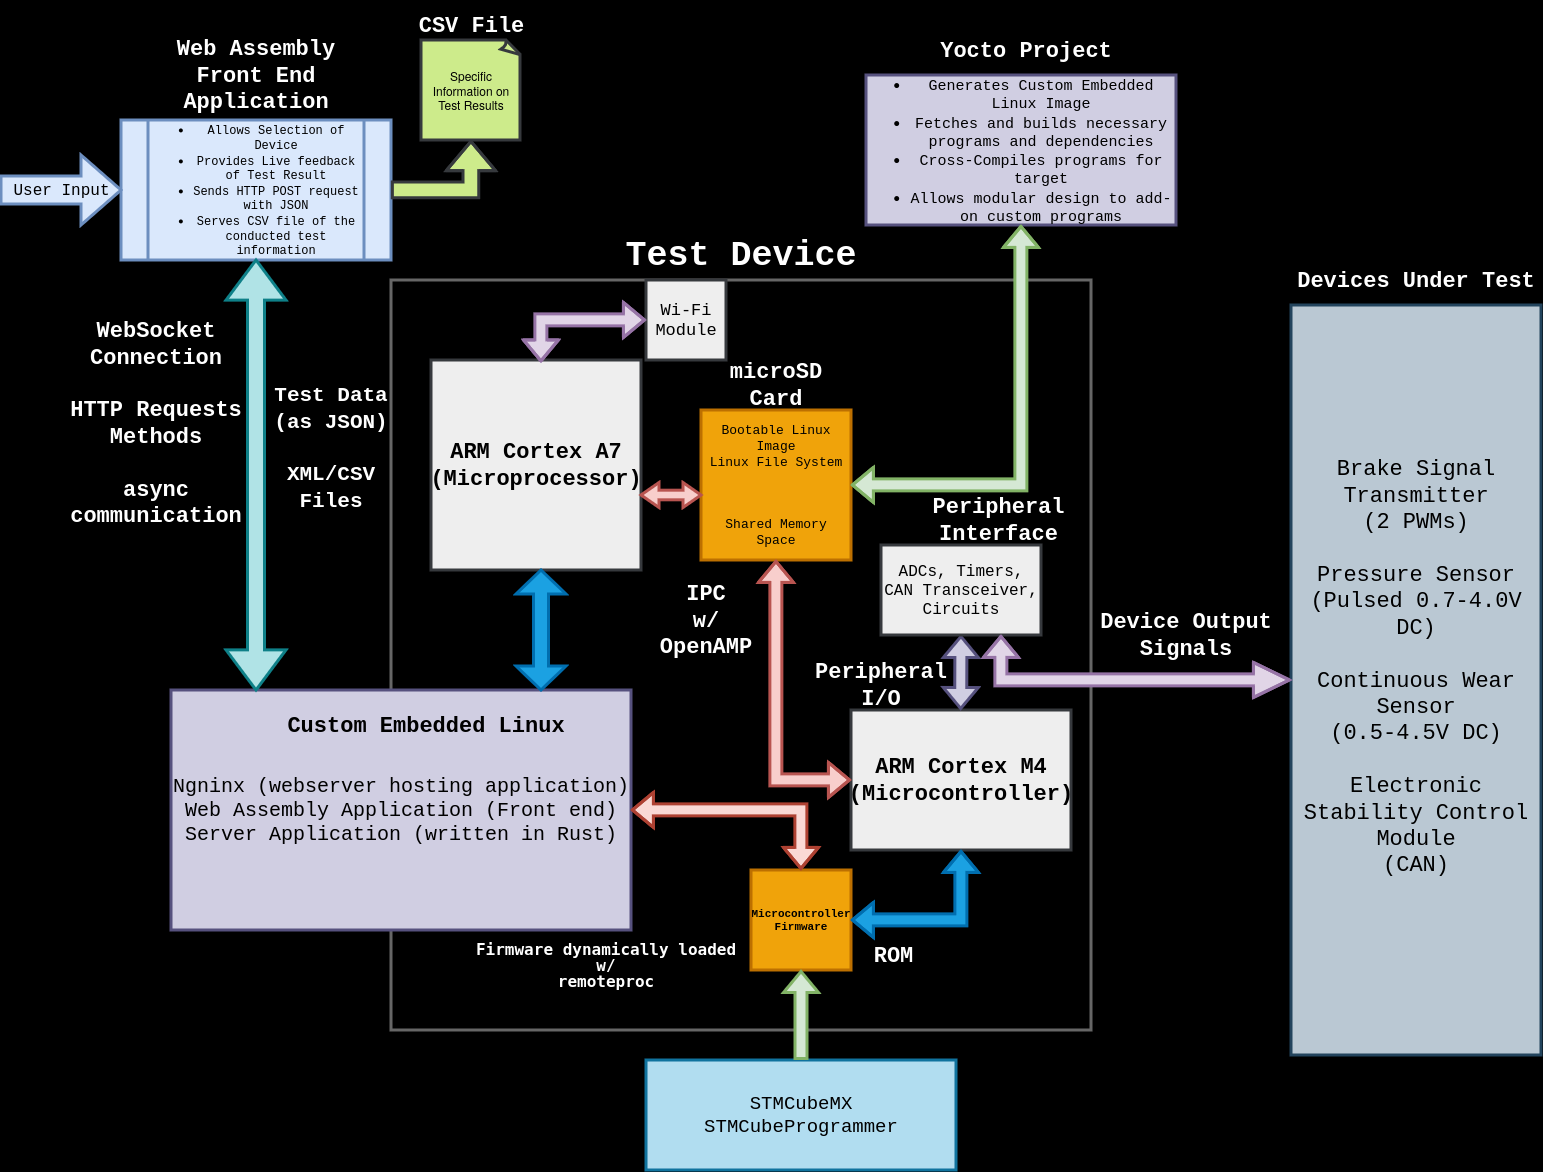
\includegraphics[width=\textwidth]{../assets/block_diagram.png}

\subsection{Specifications}
\begin{enumerate}[label=\arabic*.]
    \item Device Interfacing
        \begin{enumerate}[label=\theenumi.\arabic*]
            \item Properly read Device Signals using the ARM Cortex-M4 on the onboard 
                  microcontroller on the STM32MP157F-DK2
                \begin{itemize}
                    \item PWM duty cycle
                    \item Frequency
                    \item Voltages through an analog-to-digital converter (ADC)
                    \item CAN frames
                \end{itemize}
        \end{enumerate}

    \item Physical Components and Hardware
        \begin{enumerate}[label=\theenumi.\arabic*]
            \item Printed Circuit Board (PCB) for interfacing with DUT
            \item PCB for scaling and managing power for the DUT and to the 
                  microcontroller
            \item Enclosure for PCBs and STM32MP157F-DK2 board
        \end{enumerate}

    \item Software
        \begin{enumerate}[label=\theenumi.\arabic*]
            \item Custom embedded Linux distribution that will run on the onboard ARM 
                  Cortex-A7 microprocessor on the STM32MP157F-DK2
            \item Simple user interface on web-based application
            \item Custom Webserver to process information from web application to 
                  microcontroller
            \item Communicate collected information from ARM Cortex-M4 to ARM 
                  Cortex-A7
            \item Ability to download measured data, formatted as a CSV, through the 
                  web application
        \end{enumerate}
\end{enumerate}


\subsection{Deliverables}
The hardware component centers around custom circuit designs, featuring
\textbf{two specialized printed circuit boards}: a power management PCB that
handles voltage conversion and regulation, and a peripheral interface PCB that
manages signal routing and conditioning. Supporting these boards are
\textbf{protective enclosures} designed to house both the PCBs and the
STM32MP157F-DK2 development board, along with a comprehensive \textbf{wiring
harness system} for reliable device connections.

The software architecture comprises multiple integrated components. At its
foundation lies a \textbf{custom embedded Linux distribution} built using the
Yocto Project, which provides the operating system environment. User
interaction is handled through a \textbf{WebAssembly-based frontend interface}
that enables device selection and test control. A \textbf{Rust-based web
server} manages device communication and test execution. The system includes
specialized \textbf{ARM Cortex-M4 firmware} modules for testing various
devices: the Brake Signal Transmitter (BST) through PWM signal analysis, the
Continuous Wear Sensor (CWS) via voltage measurements, pressure sensor
validation, and Electronic Stability Control Module (ESCM) testing through CAN
communication.

The testing and documentation deliverables ensure system validation and future
maintainability. These include comprehensive \textbf{validation test results}
demonstrating compliance with manufacturer specifications, a \textbf{CSV data
export system} for maintaining test records, detailed \textbf{technical
documentation} covering system operation procedures, and organized
\textbf{source code repositories} with thorough documentation to support future
maintenance and upgrades. Together, these components form a unified testing
platform capable of handling multiple automotive sensor types while maintaining
strict compliance with ZF Group's testing requirements.

%----------------------------------------------------------------------------------------
%	Design and Implementation
% 
% * Hardware (Circuit/PCB) and device interfacing and power management
% * Enclosure Design
% * ARM Cortex-M4 Firmware
% * Embedded Linux with Yocto Project
% * Web Assembly application
% * Webserver
% * Inter-Processor Communication (IPC)
%----------------------------------------------------------------------------------------
\section{Design and Implementation}
\subsubsection{Custom Printed Circuit Board for Device interfacing and Power Management}

\subsection{Arm Cortex-M4 firmware for device Testing}

\subsection{Embedded Linux with Yocto Project}

\subsection{Custom API Web Server in Rust}

\subsection{Web Assembly Application using the Yew framework}


%----------------------------------------------------------------------------------------
%	Design Considerations 
%----------------------------------------------------------------------------------------
\subsection{Design Considerations}

\subsubsection{Public Health}

\subsubsection{Safety and Welfare}

\subsubsection{Global Impact}

\subsubsection{Cultural Impact}

\subsubsection{Social Impact}

\subsubsection{Environmental/Sustainability}

\subsubsection{Economic}


%----------------------------------------------------------------------------------------
%	Design Impacts
%----------------------------------------------------------------------------------------
\subsection{Design Impacts}

\subsubsection{Global}

\subsubsection{Economic}

\subsubsection{Environmental}

\subsubsection{Societal}


%----------------------------------------------------------------------------------------
%	Performance and Testing Analysis
%----------------------------------------------------------------------------------------
\subsection{Performance and Testing Analysis}


%----------------------------------------------------------------------------------------
%	Conclusion
%----------------------------------------------------------------------------------------
\section{Conclusion}


\end{document}
